\documentclass[12pt,a4paper]{article}
\usepackage[legalpaper, portrait, margin=3cm]{geometry}
\usepackage{fancyhdr}
\usepackage{amsmath}
\usepackage{amssymb}
\usepackage{graphicx}
\usepackage{wrapfig}
\usepackage{blindtext}
\usepackage{hyperref}
\usepackage{biblatex}

\graphicspath{ {./} }
\hypersetup{
  colorlinks=true,
  linkcolor=blue,
  filecolor=magenta,
  urlcolor=blue,
  citecolor=blue,
  pdftitle={Relatório ASA - Projeto 1 - 2022/2023},
  pdfpagemode=FullScreen,
}
\addbibresource{./bibliography.bib}

\pagestyle{fancy}
\fancyhf{}
\rhead{Grupo \textbf{al013}}
\lhead{Relatório Projeto 1 ASA 2022/2023 LEIC-A}
\cfoot{Gonçalo Bárias (103124)}

\renewcommand{\footrulewidth}{0.2pt}

\renewcommand{\labelitemii}{$\circ$}
\renewcommand{\labelitemiii}{$\diamond$}

\begin{document}
  \section{Descrição do Problema e da Solução}

  % TODO: Descrição do Problema e da Solução

  \section{Análise Teórica}

  % TODO: Análise Teórica

  Seja $N$ o número de elementos da sequência 1 e $M$ o número de elementos da sequência 2.

  \begin{itemize}
    \setlength{\itemsep}{0pt}
    \item Simples leitura do input, colocando cada elemento num vetor. Logo, $\Theta(N)$.
    \item Criação de uma lista vazia de stacks é feito em tempo constante, logo $\Theta(1)$.
    \item Cada elemento da sequência é visitado uma vez, logo $\Theta(N)$.
    \begin{itemize}
      \setlength{\itemsep}{0pt}
      \item A lista de pilhas encontra-se ordenada pelo elemento no topo da pilha, pelo que se pode aplicar o algoritmo \textit{binary search} para determinar em que pilha inserir o elemento. Logo, $O(\log N)$.
      \item Cada pilha encontra-se também ordenada, pelo que se pode determinar o índice do maior elemento menor que o elemento a inserir também pelo algoritmo \textit{binary search}. Determinar o elemento no topo da pilha é feito em tempo constante. Logo, $O(\log N)$.
      \item Obter o elemento no topo da pilha é feito em tempo constante, logo a soma à quantidade é $\Theta(1)$.
      \item Adicionar um elemento à pilha é feito também em tempo constante. Logo, $\Theta(1)$.
      \item Finalmente, adicionar uma pilha à lista é também em tempo constante. Logo, $\Theta(1)$.
    \end{itemize}
    \item A obtenção das soluções após construir a lista de pilhas, assim como a aprensen-tação dos resultados, são feitas em tempo constante. Logo, $\Theta(1)$.
  \end{itemize}

  Assim, a complexidade global da solução é $O(N \log N)$.

  Em relação à complexidade espacial, temos $\Theta(N)$, visto que cada elemento da sequência é adicionado à lista de pilhas uma e apenas uma só vez.

  \section{Avaliação Experimental dos Resultados}

  % TODO: Avaliação Experimental dos Resultados

  O programa foi executado, pelo menos 5 vezes para cada sequência, para ambos os problemas, recorrendo ao programa \href{https://github.com/sharkdp/hyperfine}{\textit{hyperfine}}.

  \begin{wrapfigure}{r}{0.4\textwidth}
    \centering
    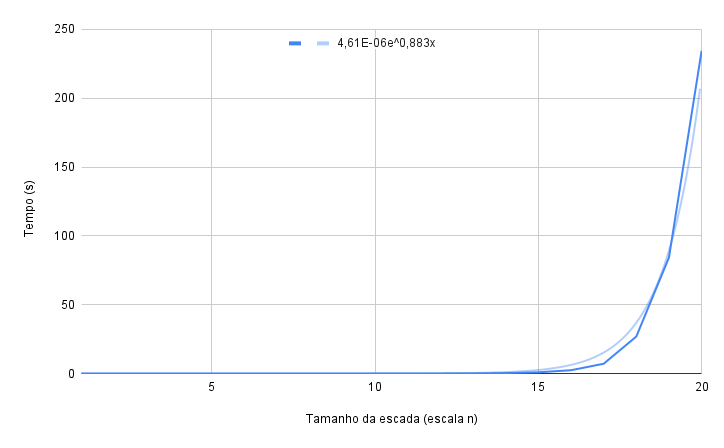
\includegraphics[width=0.4\textwidth]{report.png}
  \end{wrapfigure}

  Para o problema 2, por ser o pior caso e para simplificar a análise, tomou-se sempre $N = M$, ou seja, o mesmo número de elementos para ambas as sequências.
  Foram sempre utilizados números comuns, visto que esse é o pior caso no problema 2.
  Foram utilizadas sequências de tamanho entre 10 e 100 000 elementos, 100 para cada ordem de grandeza.
  O gráfico apresentado à direta tem uma escala $NM$ no eixo dos $xx$.
  Os dados revelam uma reta linear, comprovando que a complexidade temporal do problema é, num caso geral, $O(NM)$, tal como concluído na análise teórica.

  \section{Bibliografia}

  \printbibliography

\end{document}
Footer
